\documentclass{beamer}

\usepackage[italian]{babel}
\usepackage{enumitem}
\usepackage{ragged2e}
\usepackage{graphicx}

\usepackage[T1]{fontenc}
\usepackage[scaled=0.9]{DejaVuSansMono}

\usepackage{listings}
\lstset{
  basicstyle=\ttfamily\footnotesize,
}

\usetheme{metropolis}
\metroset{block=fill}

\title{Intelligenza Artificiale e Laboratorio}
\subtitle{Discussione laboratorio Prolog e Clingo}
\date{5 Luglio 2023}
\author{Matteo Brunello (mat. 858867)\newline Lorenzo Caresio (mat. 836021)}
\institute{Università degli Studi di Torino - Dipartimento di Informatica}

\begin{document}

    \maketitle

    \begin{frame}{Outline}
        \begin{itemize}
            \LARGE
            \item[•] Prolog
            \begin{itemize}
                \item[•] Knowledge Representation
                \item[•] Strategie informate
                \begin{itemize}
                    \item[•] Euristiche
                    \item[•] A*
                    \item[•] IDA*
                \end{itemize}
            \end{itemize}
            \item[•] Clingo
        \end{itemize}
    \end{frame}

    \section{Prolog}

    \begin{frame}{Knowledge Representation}

        \begin{columns}[c, onlytextwidth]
            \begin{column}{0.50\textwidth}

                \begin{itemize}
                    \item[•] Dominio: Trains for Europe\footnote{\url{https://trainsforeurope.eu/}}
                    \item[•] 104 stazioni
                    \item[•] 166 collegamenti
                \end{itemize}

            \end{column}

            \begin{column}{0.50\textwidth}
                \begin{figure}
                    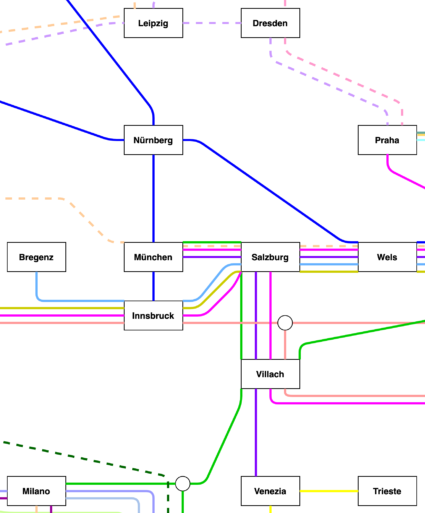
\includegraphics[height=6.5cm]{figs/domain.png}
                \end{figure}
            \end{column}
        \end{columns}

    \end{frame}

    \begin{frame}[fragile]{Knowledge Representation (II)}

        \begin{itemize}
            \Large
            \centering
            \item[•] {\tt station(city name, lat, long)}
        \end{itemize}

        \begin{lstlisting}[frame=single, language=Prolog]
...
station(wien, 48.2083537, 16.3725042).
station(linz, 48.3059078, 14.286198).
station(wels, 48.1565472, 14.0243752).
station(salzburg, 47.7981346, 13.0464806).
station(innsbruck, 47.2654296, 11.3927685).
...
        \end{lstlisting}

        \begin{figure}
                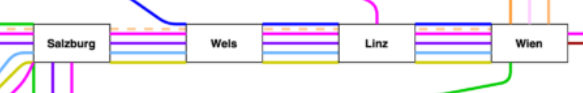
\includegraphics[height=1.5cm]{figs/stations.png}
        \end{figure}

    \end{frame}

    \begin{frame}[fragile]{Knowledge Representation (III)}

        \begin{itemize}
            \centering
        \item[•] {\tt connected(line, start\_station, next\_station, distance\_in\_km\footnote{\url{https://signal.eu.org/osm}})}
        \end{itemize}

        \begin{lstlisting}[frame=single, language=Prolog]
...
connected(nightjet_466, innsbruck, salzburg, 192).
connected(nightjet_466, salzburg, wels, 101).
connected(nightjet_466, wels, linz, 27).
connected(nightjet_466, linz, wien, 212).
connected(nightjet_465, zurich, innsbruck, 501).
connected(nightjet_465, innsbruck, graz, 732).
connected(nightjet_40466, linz, wien, 212).
connected(nightjet_40466, wels, linz, 27).
connected(nightjet_40466, salzburg, wels, 101).
connected(nightjet_40466, salzburg, munchen, 145).
connected(nightjet_40466, villach, salzburg, 181).
...
        \end{lstlisting}
    \end{frame}

    \begin{frame}[fragile]{Knowledge Representation (IV)}

        \begin{itemize}

            \item[•] Azioni:

            \begin{itemize}
                \item[•] {\tt get\_on(Line)}
                \item[•] {\tt stay\_on(City)}
                \item[•] {\tt get\_off(City)}
            \end{itemize}

            \item[•] Rappresentazione dello stato:

            \begin{itemize}
                \item[•] {\tt agent(AgentState, Position)}
                \item[•] Dove {\tt AgentState}:
                    \begin{itemize}
                        \item[•] {\tt moving(Line)}
                        \item[•] {\tt stop}
                    \end{itemize}
            \end{itemize}

        \end{itemize}

        \begin{lstlisting}[frame=single, basicstyle=\ttfamily\scriptsize]
get_on(ic_notte_799),stay_on(torino),get_off(milano),
get_on(ic_notte_795),stay_on(milano),stay_on(bologna),
get_off(roma),get_on(ic_notte_799),stay_on(roma),
get_off(salerno),get_on(ic_notte_1963),stay_on(salerno),
get_off(syracuse) % Pianificazione da Torino a Siracusa
\end{lstlisting}


    \end{frame}

    \begin{frame}{Euristiche}
        \begin{itemize}
            \item[•] Distanza euclidea: \\
                \vspace{0.2cm}
                $\sqrt{\Delta_{Lat}^2 + \Delta_{Lon}^2}$
                \vspace{0.2cm}
            \begin{itemize}
                \item[•] La distanza da gradi va portata in chilometri
            \end{itemize}

            \vspace{0.2cm}
            \hrule
            \vspace{0.2cm}

            \item[•] Distanza \textit{Haversine} (\textit{emisenoverso}): \\
                    \vspace{0.2cm}
                    $2r \sin (\sqrt{\sin^2(\frac{Lat_2 - Lat_1}{2}) + \cos(Lat_1) \cdot \cos(Lat_2) \cdot \sin^2(\frac{Lon_2 - Lon_1}{2})})$ \\
                    \vspace{0.2cm}
            \begin{itemize}
                \item[•] $r$ è il raggio del pianeta Terra in chilometri
                \item[•] I valori in gradi vanno portati in radianti
            \end{itemize}

            \vspace{0.2cm}
            \hrule
            \vspace{0.2cm}

            \item[•] Computazionalmente simili
        \end{itemize}
   \end{frame}

        \begin{frame}{Euristiche (II)}
        \begin{itemize}
            \item[•] Accuratezza:
            \begin{itemize}
                \item[•] {\tt\footnotesize euclidean\_distance(roma, budapest)} $= 960.250$ Km
                \item[•] {\tt\footnotesize \textbf{haversine\_distance}(roma, budapest)} $= 810.083$ Km (WA: $810.578$ Km)
                \item[•] Distanza calcolata con A*: 1413 Km
            \end{itemize}
            \item[•] Ammissibilità:
            \begin{itemize}
                \item[•] {\tt\footnotesize euclidean\_distance(koln, amsterdam)} $= 280.143$ Km
                \item[•] {\tt\footnotesize haversine\_distance(koln, amsterdam)} $= 214.008$ Km
                \item[•] Distanza effettiva: $258$ Km
            \end{itemize}
        \end{itemize}
   \end{frame}

    \begin{frame}{A*}
        \begin{itemize}
            \Large
            \item[•] {\tt node(State, Path, GValue, FValue)}
            \item[•] {\tt expand\_node}
            \item[•] Frontiera rappresentata come lista ordinata di nodi (nessun utilizzo di code di priorità)
        \end{itemize}
    \end{frame}

    \begin{frame}{IDA*}
        \begin{itemize}
            \item[•] Iterative deepening
            \item[•] Nuovo \textit{cutoff}: il minore tra tutti gli $f(n)$ che superano il cutoff precedente
            \item[•] \textit{Memory efficient}
            \begin{itemize}
                \item[•] Memorizza solo il \textit{cutoff} tra una iterazione e l'altra
                \item[•] \textit{Eccessivamente memory efficient}
            \end{itemize}
            \item[•] Nuovo dataset: \texttt{trainsforeurope\_limited}
            \begin{itemize}
                \item[•] Una sola linea tra una città e l'altra
                \item[•] Da 166 a 104 collegamenti
            \end{itemize}
        \end{itemize}
    \end{frame}

    \begin{frame}{Performance}
        \begin{itemize}
            \item[•] Amsterdam-München:
            \begin{itemize}
                \item[•] A*: $\approx 0.003$ secondi
                \item[•] IDA*: $\approx 0.020$ secondi
            \end{itemize}
            \item[•] Amsterdam-Siracusa:
            \begin{itemize}
                \item[•] A*: $\approx 0.048$ secondi
                \item[•] IDA*: N.D.
                \item[•] A* (limited): $\approx 0.014$ secondi
                \item[•] IDA* (limited): $\approx 15$ secondi
            \end{itemize}
            \item[•] Amsterdam-Roma:
            \begin{itemize}
                \item[•] A* (limited): $\approx 0.008$ secondi
                \item[•] IDA* (limited): $\approx 0.400$ secondi
            \end{itemize}
        \end{itemize}
    \end{frame}

    \section{Clingo}

    \begin{frame}{Predicati}
        \begin{itemize}
            \LARGE
            \item[•] \texttt{squadra/1}
            \item[•] \texttt{citta/1}
            \item[•] \texttt{stadio/2}
            \item[•] \texttt{giornata/1}
            \item[•] \texttt{match/2}
            \item[•] \texttt{assegna/2}
        \end{itemize}
    \end{frame}

    \begin{frame}{Domini}
        \LARGE
        \begin{itemize}
            \item[•] \textbf{Tiny}: 5 squadre, 10 giornate
            \item[•] \textbf{Medium}: 15 squadre, 30 giornate
            \item[•] \textbf{Real}: 20 squadre, 38 giornate
        \end{itemize}
    \end{frame}

\begin{frame}{Risultati ottenuti}
    \begin{table}[]
        \begin{tabular}{|l|l|l|l|}
        \hline
                                 & Tiny        & Medium     & Real      \\ \hline
        Nessun vincolo opzionale & $\sim$4ms   & $\sim$0.4s & $\sim$6s  \\ \hline
        Un vincolo opzionale     & $\sim$6ms   & $\sim$4s   & $\sim$30s \\ \hline
        Due vincoli opzionali    & $\sim$110ms & $\sim$4.2s & N.D.      \\ \hline
        \end{tabular}
    \end{table}
\end{frame}




\end{document}
